\documentclass{beamer}
\usepackage{ctex, hyperref}
\usepackage[T1]{fontenc}

% other packages
\usepackage{latexsym,amsmath,xcolor,multicol,booktabs,calligra}
\usepackage{graphicx,pstricks,listings,stackengine}

\author{userElaina}
\title{高可拓展性文件分类管理软件\\的设计与开源实现}
\subtitle{毕业论文答辩}
\institute{航空航天器械清洁学院}
\date{2023年06月04日}
\usepackage{JilinUniv}

% defs
\def\cmd#1{\texttt{\color{red}\footnotesize $\backslash$#1}}
\def\env#1{\texttt{\color{blue}\footnotesize #1}}
\definecolor{deepblue}{rgb}{0,0,0.5}
\definecolor{deepred}{rgb}{0.6,0,0}
\definecolor{deepgreen}{rgb}{0,0.5,0}
\definecolor{halfgray}{gray}{0.55}

\lstset{
    basicstyle=\ttfamily\small,
    keywordstyle=\bfseries\color{deepblue},
    emphstyle=\ttfamily\color{deepred},    % Custom highlighting style
    stringstyle=\color{deepgreen},
    numbers=left,
    numberstyle=\small\color{halfgray},
    rulesepcolor=\color{red!20!green!20!blue!20},
    frame=shadowbox,
}


\begin{document}

\kaishu
\begin{frame}
    \titlepage
    \begin{figure}[htpb]
        \begin{center}
            
\includegraphics[width=0.15\linewidth]{pic/Jilin_University_Logo.eps}
        \end{center}
    \end{figure}
\end{frame}

\begin{frame}
    \tableofcontents[sectionstyle=show,subsectionstyle=show/shaded/hide,subsubsectionstyle=show/shaded/hide]
\end{frame}


\section{背景和总览}

\begin{frame}{混乱的文件}
    % From thuthesis user guide.
    \begin{minipage}[r]{0.3\linewidth}
        \medskip
        %\hspace{2cm}
        \begin{figure}[h]
            \centering
            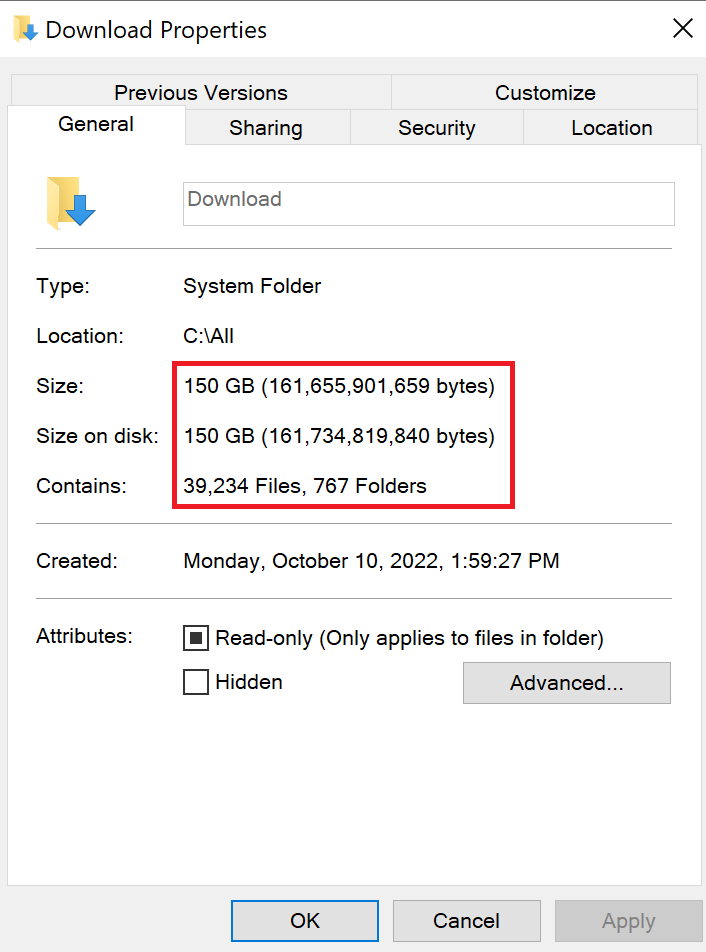
\includegraphics[height=.6\textheight]{pic/down.png}
        \end{figure}
    \end{minipage}\hspace{1cm}
    \begin{minipage}[c]{0.5\linewidth}
        \medskip
        %\hspace{2cm}
        \begin{figure}[h]
            \centering
            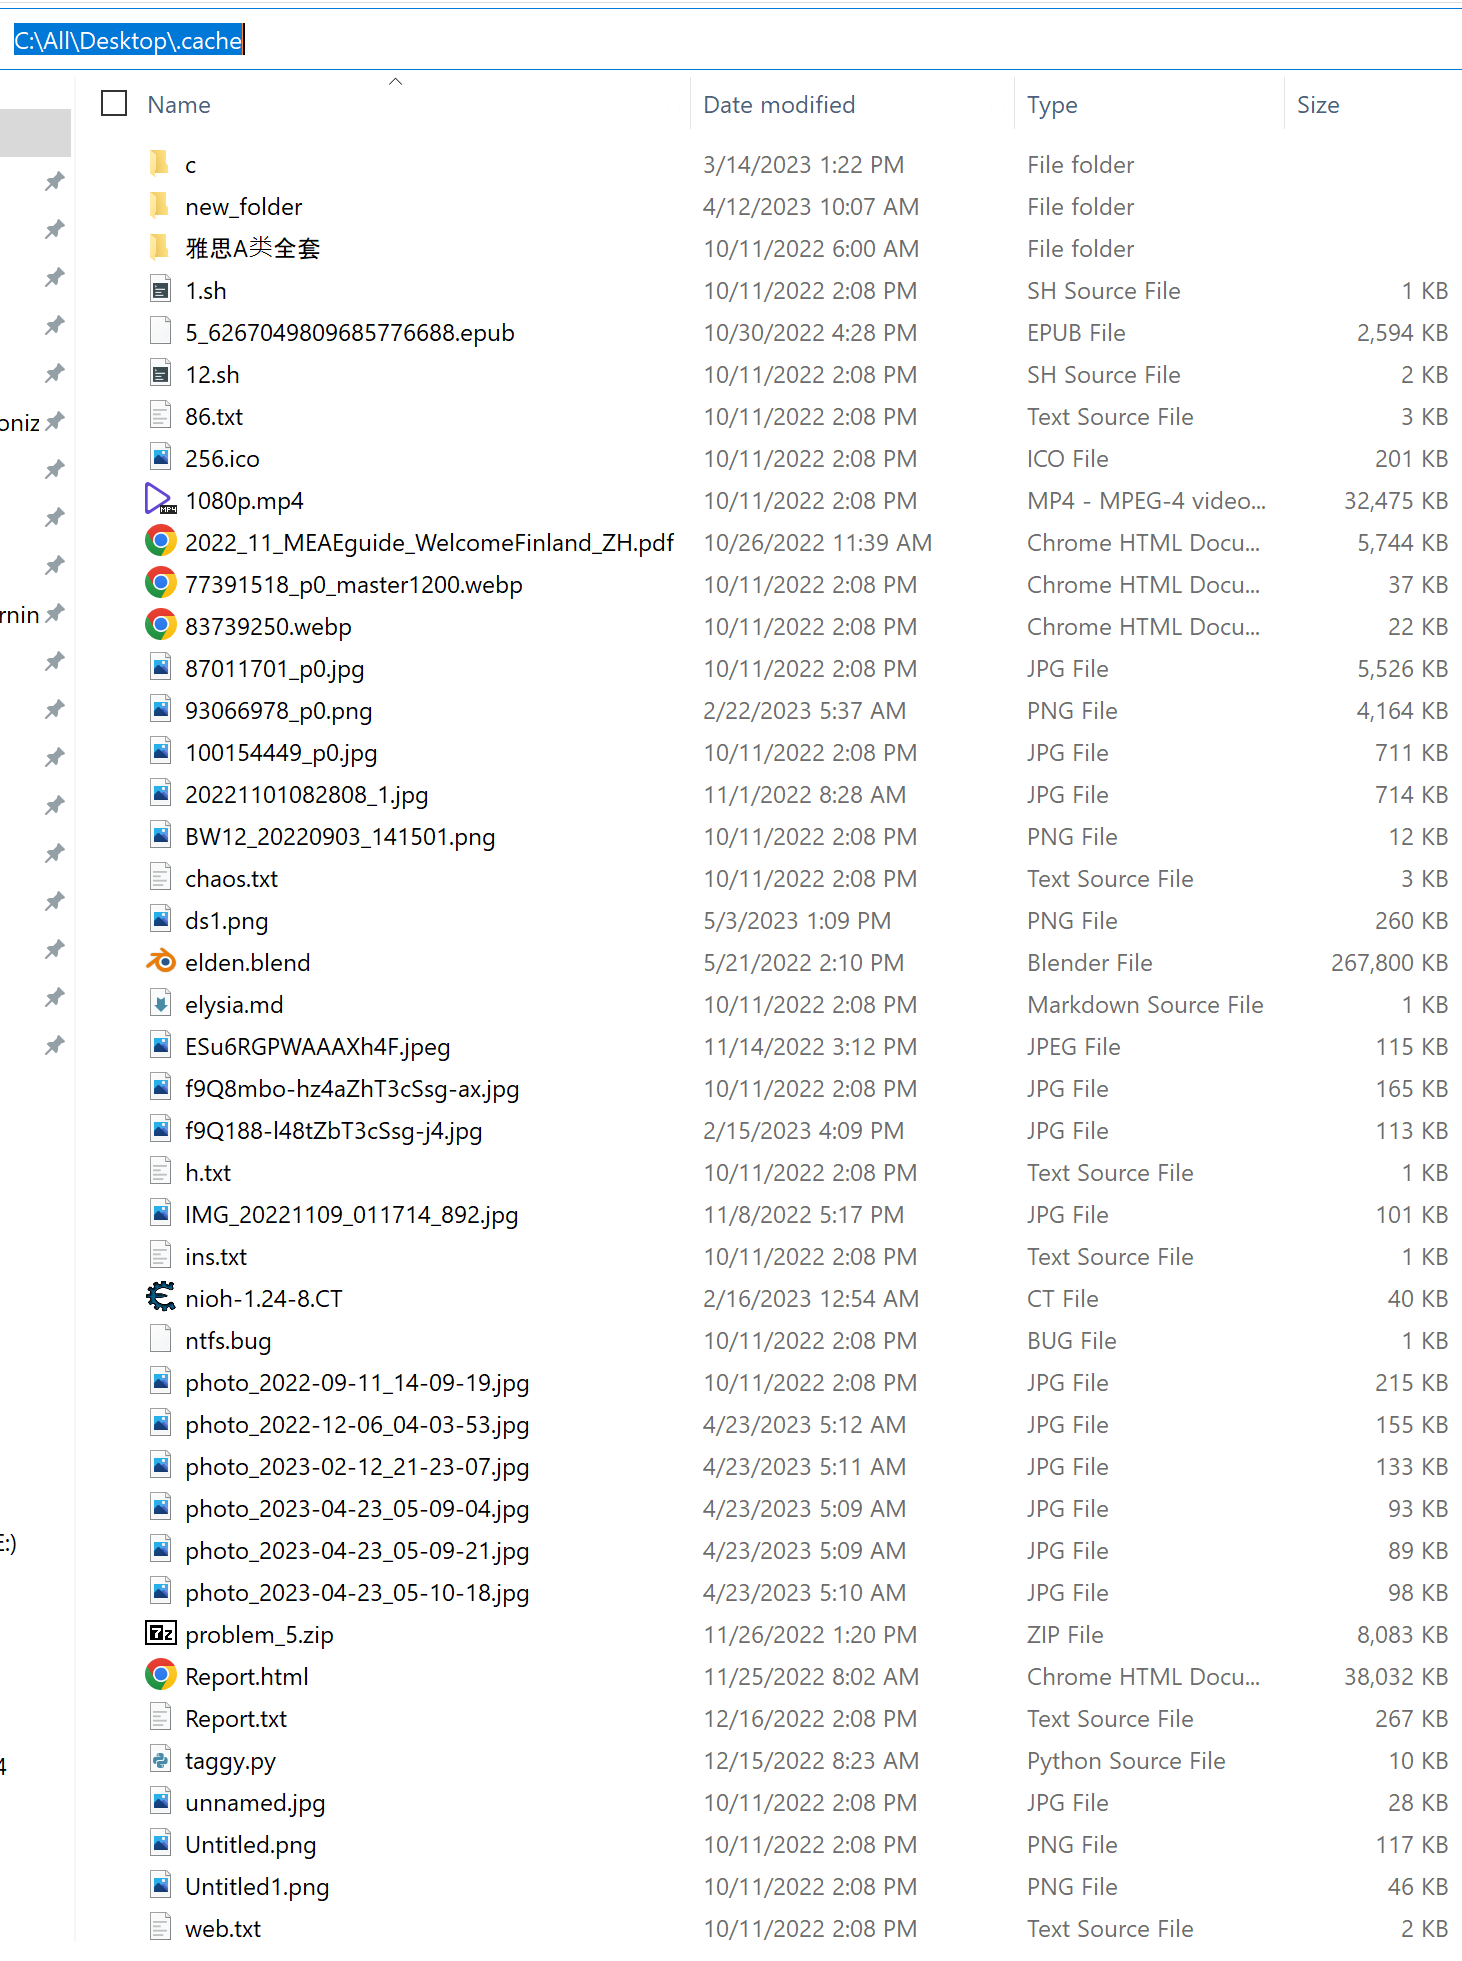
\includegraphics[height=.6\textheight]{pic/cache.png}
        \end{figure}
    \end{minipage}
\end{frame}

\begin{frame}{开发总览}
    \begin{itemize}[<+-| alert@+>] % 当然,除了alert,手动在里面插 \pause 也行
        \item 开发语言:Python 和 C++。
        \item 开发模型:迭代模型。
        \item 工具和库:OpenCV,FFmpeg,GoogLeNet。
        \item 技术:散列,编译原理,粒子群优化。
    \end{itemize}
\end{frame}

\section{设计和实现}

\begin{frame}
    \begin{itemize}[<+-| alert@+>]
        \item 常量和工具。
        \item 插件类。
        \item 事件驱动器。
        \item 默认插件和可选插件。
    \end{itemize}
\end{frame}

\begin{frame}
    \begin{figure}[h]
        \centering
        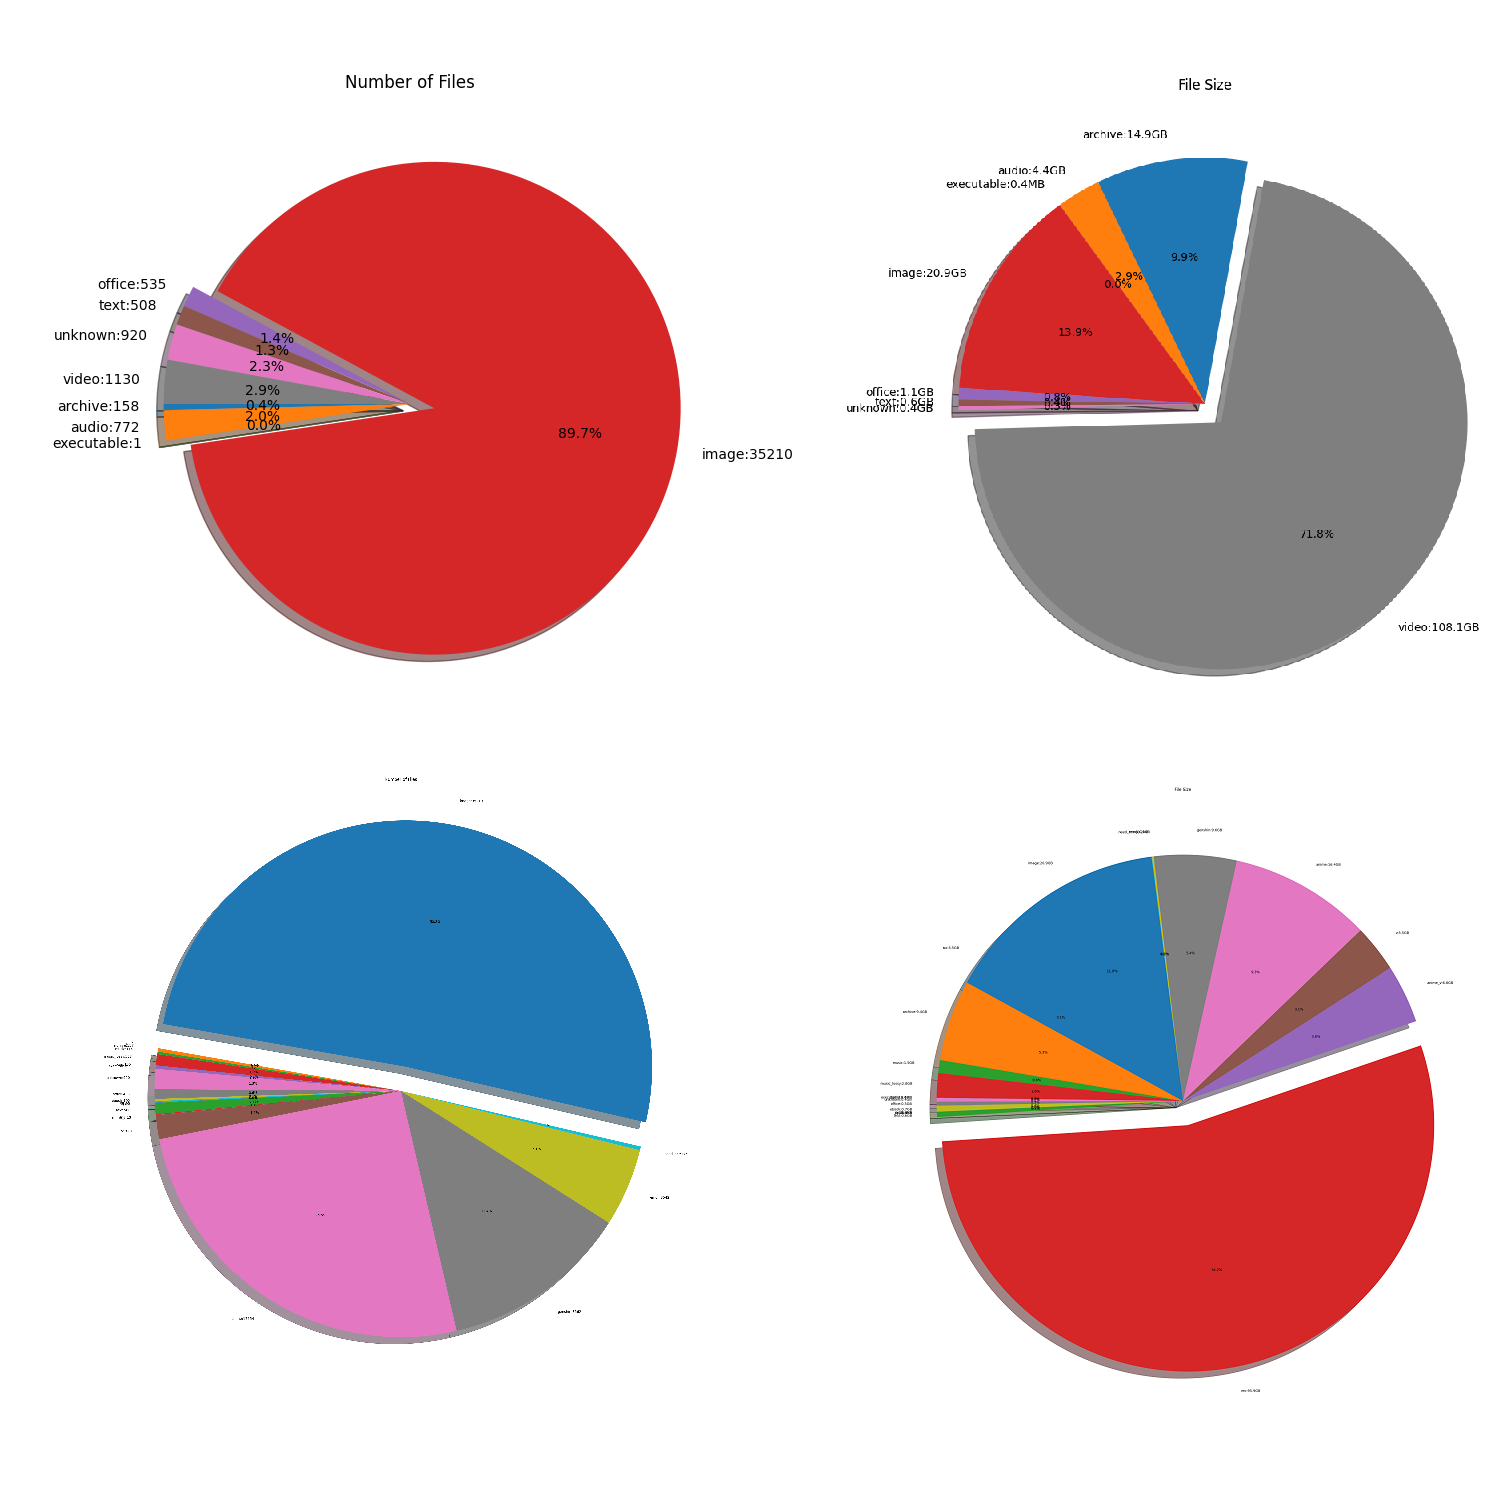
\includegraphics[height=.7\textheight]{pic/pie4.png}
        \caption{文件信息统计插件}
    \end{figure}
\end{frame}

\begin{frame}
    \begin{itemize}
        \item\begin{equation*}
            \begin{aligned}
                E &\to {\rm word},\\
                E &\to \sim E,\\
                E &\to (E),\\
                E &\to E | E,\\
                E &\to E \& E.\\
            \end{aligned}
        \end{equation*}
        \item 基于 PyParsing 的递归下降集合运算解释器插件
    \end{itemize}
\end{frame}

\begin{frame}
    \begin{figure}[h]
        \centering
        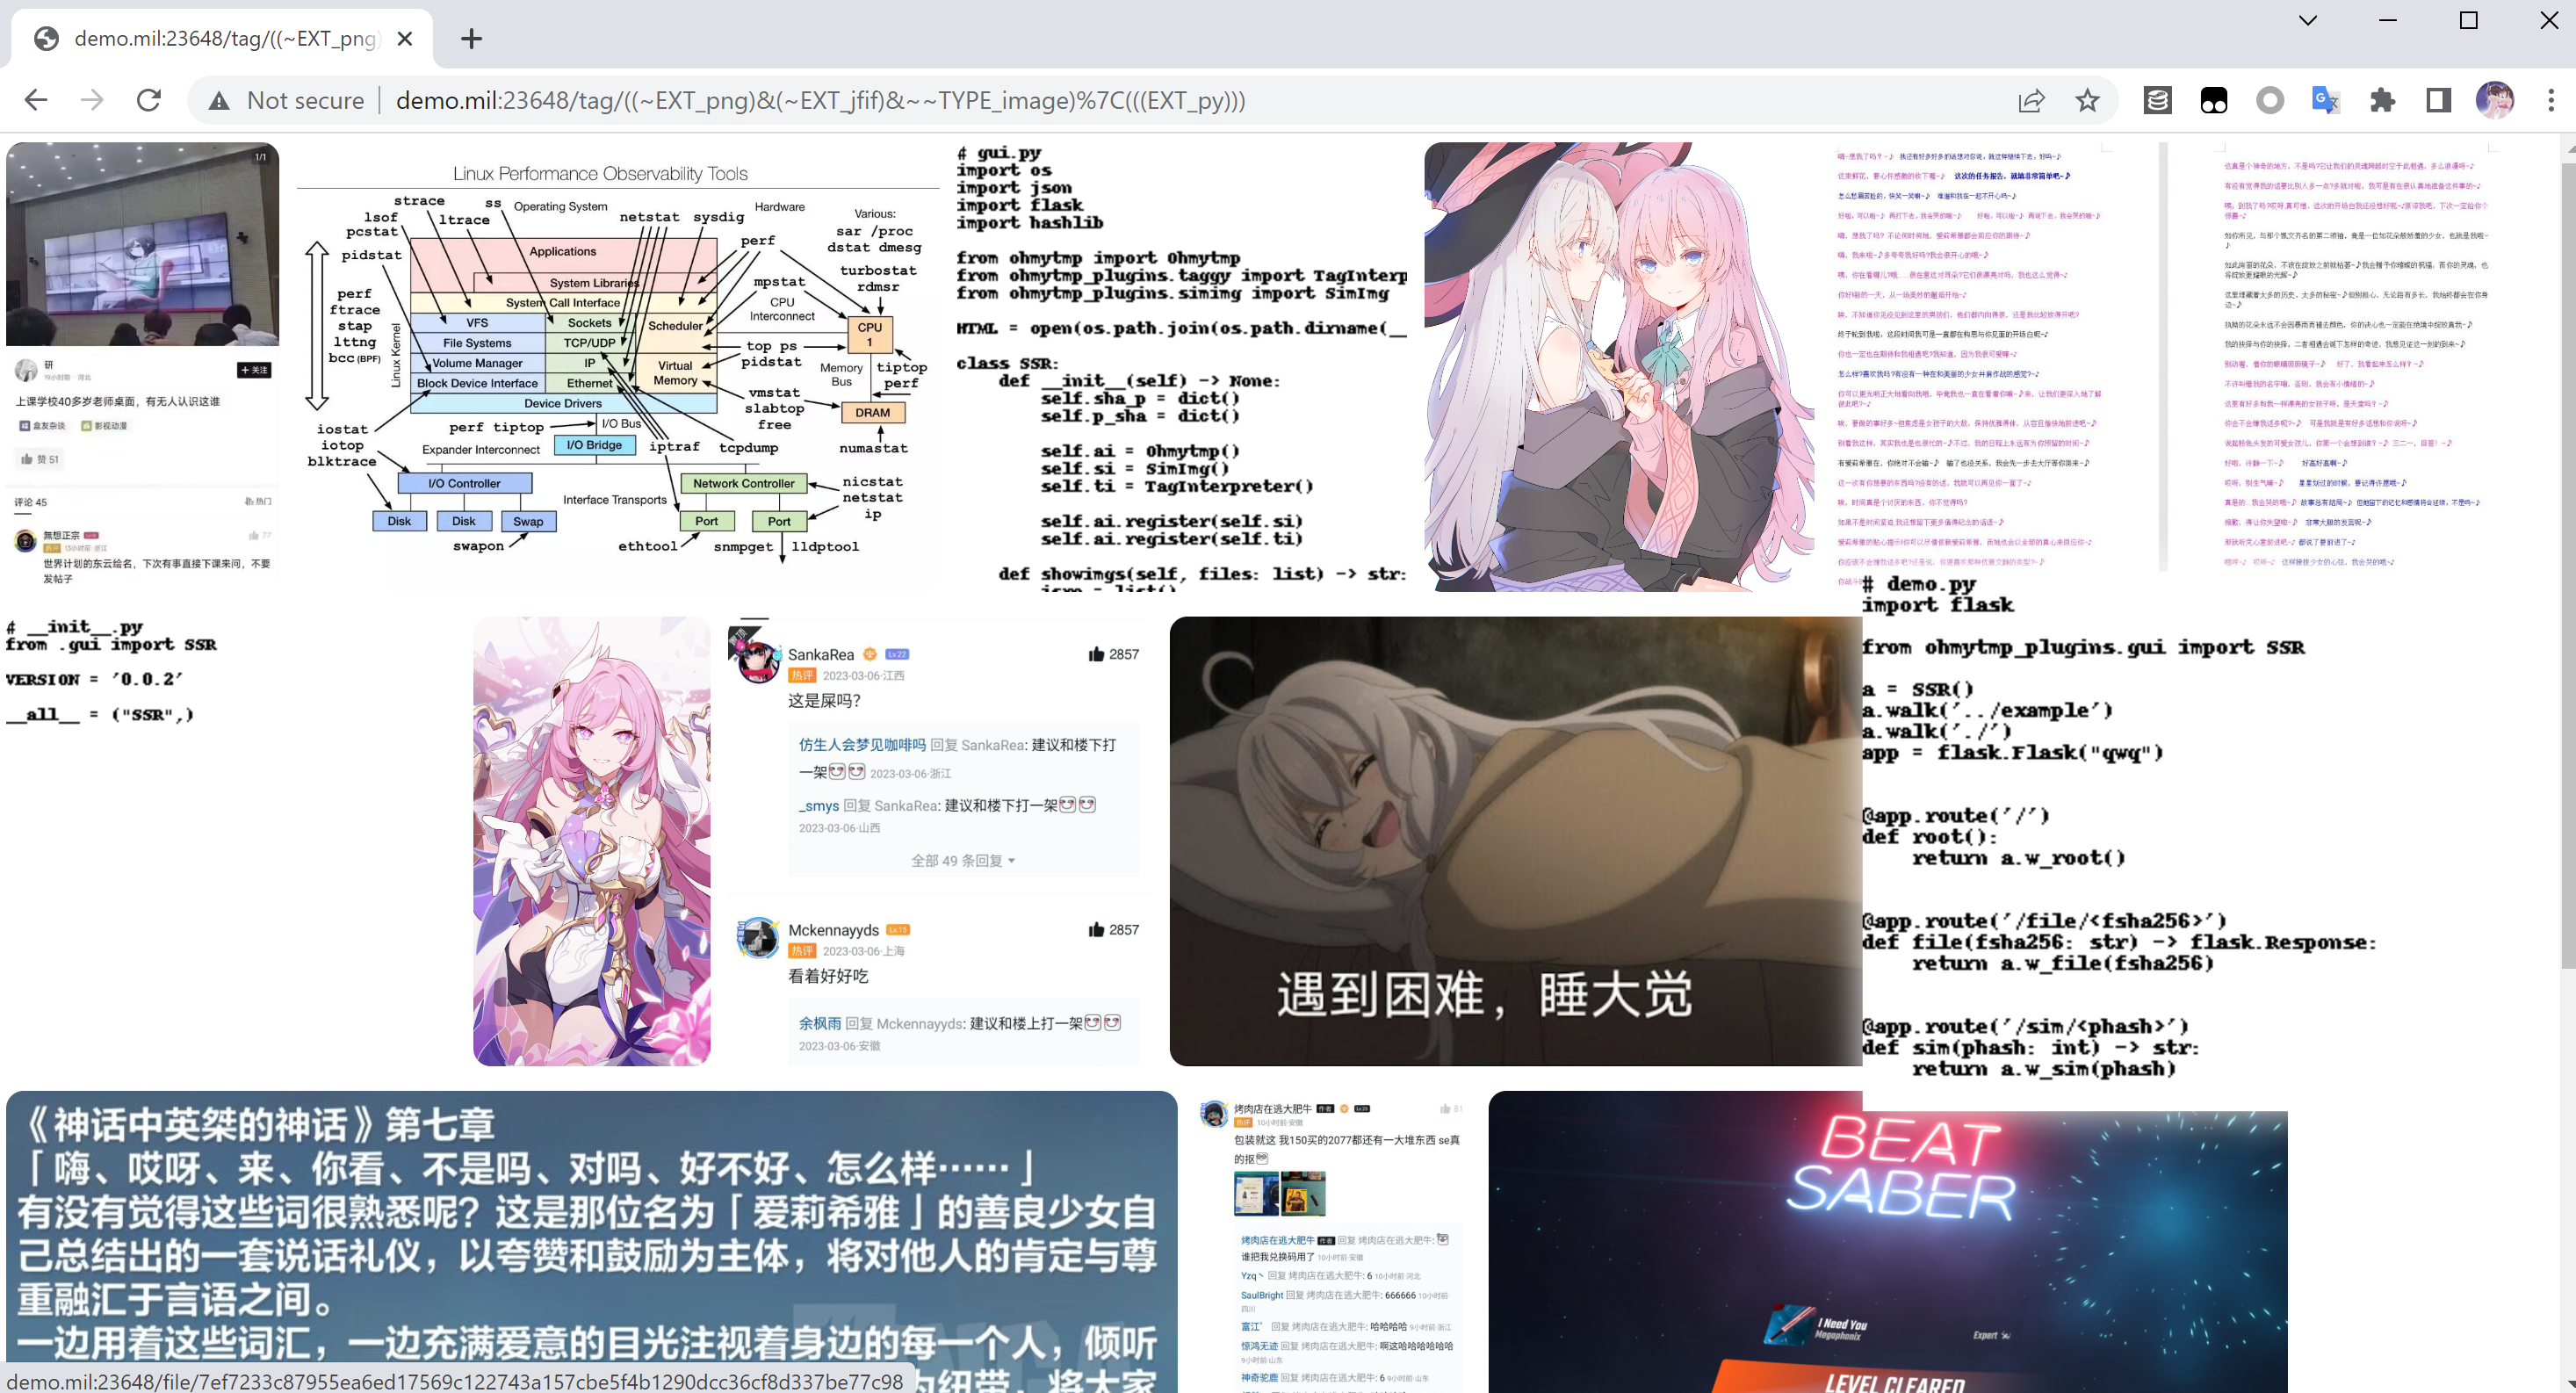
\includegraphics[height=.6\textheight]{pic/flask2.png}
        \caption{基于 Flask 的 GUI 插件:\\ \tt{((\textasciitilde EXT\_png)\&(\textasciitilde EXT\_jfif)\&\textasciitilde\textasciitilde TYPE\_image)|(((EXT\_py)))|TYPE\_image}}
    \end{figure}
\end{frame}

\begin{frame}
    \begin{figure}[l]
        \centering
        
\includegraphics[height=.5\textheight]{pic/pso.png}
        \caption{基于粒子群优化的子图匹配插件}
    \end{figure}
\end{frame}

\begin{frame}
    \begin{figure}[l]
        \centering
        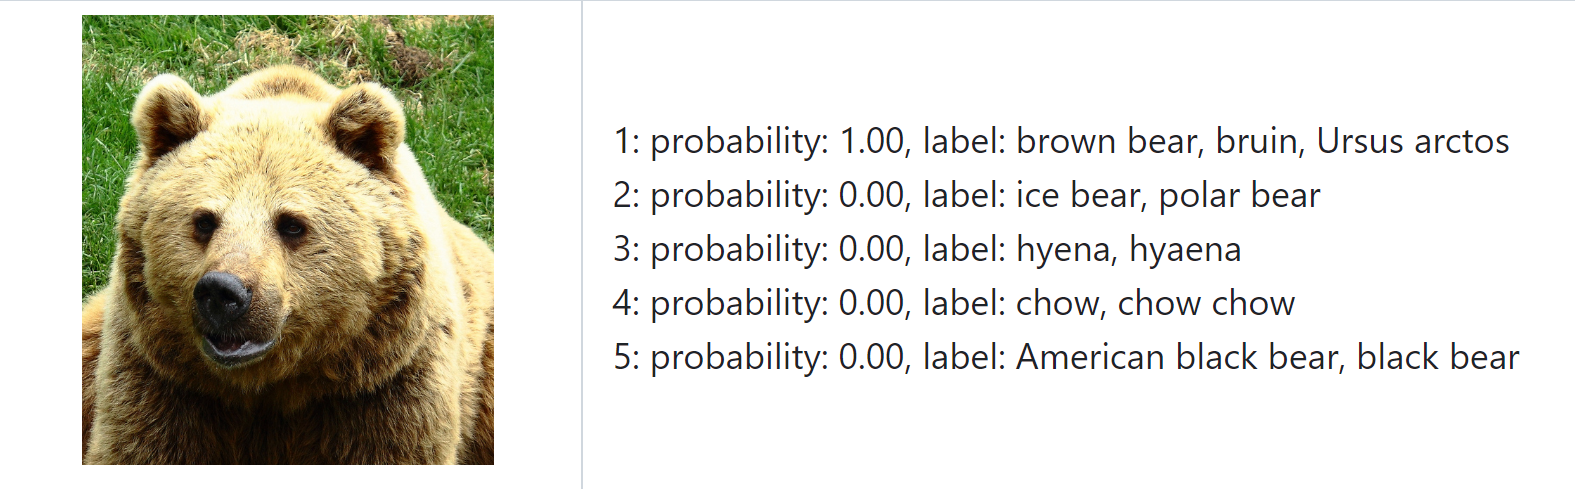
\includegraphics[height=.4\textheight]{pic/ggnet.png}
        \caption{基于 GoogLeNet 的图像标签生成插件}
    \end{figure}
\end{frame}

\section{总结}

\begin{frame}{总结}
    \begin{itemize}[<+-| alert@+>] % 当然,除了alert,手动在里面插 \pause 也行
        \item 参考文献 65 篇。
        \item Oh My ZSH! 与 Oh My \tt{/tmp} .
        \item 3 Pull Requests (2 Merge), 1 Issue.
        \item GitHub: \url{https://github.com/ohmytmp} .
        \item PyPi.
        \item 个人需求驱动。
    \end{itemize}
\end{frame}

\begin{frame}
    \begin{center}
        {\Huge\calligra Thanks!}
    \end{center}
\end{frame}

\end{document}